\documentclass[norsk,a4paper,12pt]{article}
\usepackage[utf8]{inputenc}
\usepackage{graphicx} %for å inkludere grafikk
\usepackage{verbatim} %for å inkludere filer med tegn LaTeX ikke liker
\usepackage{tabularx}
\usepackage{booktabs}
\usepackage{amsmath}
\usepackage{float}
\usepackage{color}
\usepackage{listings}
\usepackage{hyperref}
\usepackage{amsmath}

\lstset{language=c++}
\lstset{basicstyle=\small}
\lstset{backgroundcolor=\color{white}}
\lstset{frame=single}
\lstset{stringstyle=\ttfamily}
\lstset{keywordstyle=\color{red}\bfseries}
\lstset{commentstyle=\itshape\color{blue}}
\lstset{showspaces=false}
\lstset{showstringspaces=false}
\lstset{showtabs=false}
\lstset{breaklines}
\lstset{postbreak=\raisebox{0ex}[0ex][0ex]{\ensuremath{\color{red}\hookrightarrow\space}}}
\usepackage{titlesec}

\setcounter{secnumdepth}{4}

\titleformat{\paragraph}
{\normalfont\normalsize\bfseries}{\theparagraph}{1em}{}
\titlespacing*{\paragraph}
{0pt}{3.25ex plus 1ex minus .2ex}{1.5ex plus .2ex}


\title{FYS4411 - Computational Physics II\\\vspace{2mm} \Large{Project 1}}
\author{\large Dorthea Gjestvang\\ Even Marius Nordhagen}
\date\today
\begin{document}

\maketitle
\begin{abstract}
Write the abstract here
\par 

\end{abstract}


\begin{itemize}
\item Github repository containing programs and results are in: \url{https://github.com/evenmn/FYS4411/tree/master/Project%201}
\end{itemize}


\section{Introduction}
Introduction

\section{Theory}
We study a system of $N$ bosons trapped in a harmonic oscillator with the Hamiltonian given by 
\begin{equation}
\hat{H}=\sum_i^N\bigg(-\frac{\hbar^2}{2m}\nabla_i^2+V_{ext}(\vec{r}_i)\bigg)+\sum_{i<j}^NV_{int}(\vec{r}_i,\vec{r}_j)
\label{eq:Hamilton}
\end{equation}
with $V_{ext}$ as the external potential, which is the harmonic oscillator potential,
and $V_{int}$ as the interaction term. The interaction will in the first place be ignored, and is specified later. We will consider a harmonic oscillator which can either be spherical (all dimensions have the same scales) or elliptical (the vertical dimension has a different frequency from the horizontals),
\begin{equation}
\label{eq:V_ext}
V_{ext}(\vec{r})=
\begin{cases} 
   \frac{1}{2}m\omega_{HO}^2\vec{r}^2 & \text{(Spherical)} \\
   \frac{1}{2}m[\omega_{HO}^2(x^2 + y^2) + \omega_z^2z^2] & \text{(Elliptical)}.
\end{cases}
\end{equation}

The trial wavefunction is on the form 
\begin{equation}
\Psi_T(\vec{r}_1, \vec{r}_2, ..., \vec{r}_N, \alpha, \beta)=\prod_i^Ng(\alpha, \beta, \vec{r}_i)\prod_{i<j}f(a,r_{ij})
\label{eq:WF}
\end{equation}
where $r_{ij}=|\vec{r}_i-\vec{r}_j|$ and $g$ is assumed to be an exponential function,
\begin{equation}
g(\alpha, \beta, \vec{r}_i)=\exp[-\alpha(x_i^2+y_i^2+\beta z_i^2)],
\end{equation}
which is practical since
\begin{equation}
\prod_i^Ng(\alpha, \beta, \vec{r}_i)=\exp\Big[-\alpha\sum_{i=1}^N(x_i^2+y_i^2+\beta z_i^2)\Big].
\end{equation}
$\alpha$ is a variational parameter that we later use to find the energy minimum, and $\beta$ is a constant. This is also the form of the exact ground state wave function for a harmonic oscillator, so by choosing the correct $\alpha$, we will find the exact ground state energy (when $V_{int}$ is ignored). The $f$ presented above is the correlation wave function, which is 
\begin{equation}
f(a,r_{ij})=
\begin{cases} 
   0 & r_{ij} \leq a \\
   \left(1-\frac{a}{r_{ij}}\right) & r_{ij} > a.
\end{cases}
\end{equation}
The first case we will take into account is when $a=0$, such that the corretation term is 1. 

We want to calculate the local energy as a function of $\alpha$, and then use Variational Monte Carlo (VMC) described in section \ref{VMC}. For the non-interacting case, the analytical expression for one particle in a harmonic oscillator is well-known and reads
\begin{equation}
E = \hbar\omega(n + dim/2)
\label{Energy_exact}
\end{equation}
where $n$ is the energy level and $dim$ is number of dimensions. In this project we will study the ground state only, such that $n=0$. The local energy is
\begin{equation}
E_L(\vec{r})=\frac{1}{\Psi_T(\vec{r})}\hat{H}\Psi_T(\vec{r})
\label{eq:Local_energy}
\end{equation}
which gives the following results considering $a=0$:

INSERT ANALYTICAL EXPRESSIONS FROM A

For $a\neq0$ it gets rather more complicated, because we need to deal with the correlation term as well. By defining
\begin{equation}
f(a, r_{ij})=\exp{\bigg(\sum_{i<j}u(r_{ij})\bigg)}
\end{equation}
and doing a change of variables
\begin{equation}
\frac{\partial}{\partial \vec{r}_k}=\frac{\partial}{\partial \vec{r}_k}\frac{\partial r_{kj}}{\partial r_{kj}}=\frac{\partial r_{kj}}{\partial \vec{r}_k}\frac{\partial}{\partial r_{kj}}=\frac{(\vec{r}_k-\vec{r}_j)}{r_{kj}}\frac{\partial}{\partial r_{kj}}
\end{equation}
one will end up with
\begin{align}
E_L=\sum_k\Bigg(-\frac{1}{2}\bigg(&4\alpha^2\Big(x_k^2+y_k^2+\beta^2z_k^2-\frac{1}{\alpha}-\frac{\beta}{2\alpha}\Big)\notag\\
&-4\alpha\sum_{j\neq k}(x_k, y_k, \beta z_k)\frac{(\vec{r}_k-\vec{r}_j)}{r_{kj}}u'(r_{kj})\\
&+\sum_{ij\neq k}\frac{(\vec{r}_k-\vec{r}_j)(\vec{r}_k-\vec{r}_i)}{r_{ki}r_{kj}}u'(r_{ki})u'(r_{kj})\notag\\
&+\sum_{j\neq k}\Big(u''(r_{kj})+\frac{2}{r_{kj}}u'(r_{kj})\Big)\bigg)+V_{ext}(\vec{r}_k)\Bigg).\notag
\label{EL_total}
\end{align}
This is not a pretty expression, but hopefully it will give us the correct answers. We could also split up the local energy expression 
\begin{equation}
E_{L,i}=-\frac{\hbar^2}{2m}\frac{\nabla_i^2\Psi_T}{\Psi_T}+V_{ext}(\vec{r}_i)=E_{k,i}+E_{p,i}
\end{equation}
and calculate the local energy with a numerical approach where the second derivative can be approximated by the three-point formula:
\begin{equation}
f''(x)\simeq\frac{f(x+h)-2f(x)+f(x-h)}{h^2}.
\end{equation}
In our case the position is a three dimensional vector, so we need to handle each dimension separately. Both the analytical and the numerical local energy are implemented, and in section \ref{CPU}, the CPU time for the analytical and numerical approach are compared for a various number of particles. 

The most interesting and realistic case is when the interaction is included, so let us now set it to a so-called hard-sphere potential
\begin{equation}
V_{int}(\vec{r}_i, \vec{r}_j)=
\begin{cases} 
   0 & \text{if}\quad |\vec{r}_i-\vec{r}_j| \geq a \\
   \infty & \text{if}\quad |\vec{r}_i-\vec{r}_j| < a.
\end{cases}
\end{equation}
which ensures that the particles are separated by a distance $a$. The local energy is slightly changing, because we need to add the interaction potential to it as well. 

For the case when we have elliptical harmonic oscillator potential, we can obtain a quite simple expression for the Hamiltonian when scaling with respect to $\hbar\omega_{HO}$ (something we actually already have done with the energy). The expression we get is
\begin{equation}
H=\sum_i\bigg(\frac{1}{2}\Big(-\nabla^2 + x_i^2 + y_i^2 + \gamma^2z_i^2\Big)\bigg)+\sum_{i<j}V_{int}(\vec{r}_i,\vec{r}_j)
\end{equation}
where
\begin{equation*}
\gamma=\frac{\omega_z}{\omega_{HO}}.
\end{equation*}
This quantity is equivalent to $\beta$, see Appendix B to see how this expression is derived. 

\subsection{One-body density}
In many cases it is convenient to know the positions of the particles, but with many particles the positions itself will be overwhelming and not really give us a good picture. Instead of presenting the positions, the density of particles can give us a good overview of where the particles can be found. In this project we will study the radial density, and find the particle densities at various distances from origin. We do this by dividing the volume where the particles can be found in multiple bins and counting the number of particles in the bin. Thereafter the number of particles in each bin needs to be divided by the area of the bin, which will be a sphere surface in our case. 

\section{Methods}
\subsection{Variational Monte Carlo}\label{VMC}
Variational Monte Carlo (VMC) is a widely used method for approximating the ground state of a quantum system. The method is based on Markov chains, and move a particle (or a set of particles) one step for each cycle, i.e.
\begin{equation}
\vec{R}_{new} = \vec{R} + r\cdot \text{step}.
\end{equation}
Both the direction and the change in position are randomly chosen, so with a plain VMC implementation the particles will move randomly and independently of each other. We are going to use the Metropolis algorithm in addition to the VMC, which accepts or rejects moves based on the probability ratio between the old and the new position. This makes the system approach the most likely state, and the idea is that after a certain number of cycles the system will be in the most likely state. 

\subsection{Metropolis Algorithm}
As mentioned above the task of the Metropolis algorithm is to move the system against the most likely state. The standard algorithm, here named brute force, is the simplest one, and does not deal with the transition probabilities. The modified Metropolis-Hastings algorithm includes, on the other hand, the transition probabilities and will be slightly more time consuming per cycle. We expect the latter to converge faster to the most likely state. 

The foundation of the Metropolis algorithm is that the probability for a system to undergo a transition from state $i$ to state $j$ is given by the transition probability multiplied by the acceptance probability
\begin{equation}
W_{i\rightarrow j} = T_{i \rightarrow j}\cdot A_{i \rightarrow j}
\end{equation}
where $T_{i \rightarrow j}$ is the transition probability and $A_{i \rightarrow j}$ is the acceptance probability. Built on this, the probability for being in a state $i$ at time (step) $n$ is
\begin{equation}
P_i^{(n)} = \sum_j\bigg[P_j^{(n-1)}T_{j \rightarrow i}A_{j \rightarrow i} + P_i^{(n-1)}T_{i \rightarrow j}(1-A_{i \rightarrow j})\bigg]
\end{equation}
since this can happend in two ways. One can start in this state $i$ at time $n-1$ and be rejected or one can start in another state $j$ at time $n-1$ and complete an accepted move to state $i$. In fact $\sum_j T_{i \rightarrow j} =1$, so we can rewrite this as 
\begin{equation}
P_i^{(n)} = P_i^{(n-1)} + \sum_j\bigg[P_j^{(n-1)}T_{j \rightarrow i}A_{j \rightarrow i} - P_i^{(n-1)}T_{i \rightarrow j}A_{i \rightarrow j}\bigg].
\end{equation}
When the times goes to infinity, the system will approach the most likely state and we will have $P_i^{(n)} = p_i$, which requires
\begin{equation}
\sum_j\bigg[p_jT_{j \rightarrow i}A_{j \rightarrow i} - p_iT_{i \rightarrow j}A_{i \rightarrow j}\bigg]=0.
\end{equation}
Rearranging, we obtain a quite useful result
\begin{equation}
\frac{A_{j\rightarrow i}}{A_{i\rightarrow j}}=\frac{p_iT_{i\rightarrow j}}{p_jT_{j\rightarrow i}}
\end{equation}

\subsubsection{Brute force}
In the brute force Metropolis algorithm we want to check if the new position is more likely than the current position, and for that we calculate the probabilities $P(\vec{R})=|\Psi_T(\vec{R})|^2$ for both positions. We get rid off the transition probabilities setting $T_{i\rightarrow j}=T_{j\rightarrow i}$, and then end up with the plain ratio
\begin{equation}
w=\frac{P(\vec{R}_{new})}{P(\vec{R})}=\frac{|\Psi_T(\vec{R}_{new})|^2}{|\Psi_T(\vec{R})|^2}.
\end{equation}
$w$ will be larger than one if the new position is more likely than the current, and smaller than one if the current position is more likely than the new one. Metropolis handle this by accepting if the ratio $w$ is larger than a random number $r$ in the interval $[0,1]$, and rejecting if not:
\begin{equation}
\text{New position: }
\begin{cases} 
   \text{accept} & \text{if}\quad w > r \\
   \text{reject} & \text{if}\quad w \leq r.
\end{cases}
\end{equation}

\subsubsection{Importance sampling}
The importance sampling technique is often refered to as Metropolis-Hastings algorithm. The approach is the same as for the brute force Metropolis algorithm, but we will end ut with a slightly more complicated acceptation criteria. To understand the details, we need to begin with the Fokker-Planck equation, which describes the time-evolution of the probability density function $P(R,t)$. In one dimension it reads
\begin{equation}
\frac{\partial P(R,t)}{\partial t} = D\frac{\partial}{\partial R}\bigg(\frac{\partial}{\partial R} - F\bigg)P(R,t).
\end{equation}
where $F$ is the drift force and $D$ is the diffusion coefficient. Even though the probability density function can give a lot of useful information, an equation describing the motion of a such particle would be more appropriate for our purposes. Fortunately this equation exists, and satisfies the Fokker-Planck equation. The Langevin equation can be written as
\begin{equation}
\frac{\partial R(t)}{\partial t}=DF(R(t)) + \eta
\end{equation}
where $\eta$ can be considered as a random variable. This differential equation can be solved by applying the forward Euler method and introducing gaussian variables $\xi$
\begin{equation}
R_{new} = R + DF(R)\Delta t + \xi\sqrt{\Delta t}
\end{equation}
which will be used to update the position. Moreover we also need to update the acceptance criteria since we no longer ignore the transition probabilities. With the Fokker-Planck equation as base, the transition probabilities are given by Green's function
\begin{align}
T_{R\rightarrow R_{new}}&=G(R_{new},R,\Delta t)\notag\\
&=\frac{1}{(4\pi D\Delta t)^{3N/2}}\exp[-(R_{new} - R - D\Delta tF(R))^2/4D\Delta t] 
\end{align}
and the acceptance criteria becomes
\begin{equation}
r<\frac{G(R,R_{new},\Delta t)|\Psi_T(R_{new})|^2}{G(R_{new},R,\Delta t)|\Psi_T(R)|^2}.
\end{equation}

\subsection{Minimization methods}
When the interaction term is excluded, we know which $\alpha$ that corresponds to the energy minima, and it is in principle no need to try different $\alpha$'s. However, sometimes we have no idea where to search for the minimum point, and we need to try various $\alpha$ values to determine the lowest energy. If we do not know where to start searching, this can be a time consuming activity. Would it not be nice if the program could do this for us?

In fact there are multiple techniques for doing this, where the most complicated ones obviously also are the best. Anyway, in this project we will have good initial guesses, and are therefore not in need for the most fancy algorithms. 

\subsubsection{Gradient descent}
Perhaps the simplest and most intuitive method for finding the minima is the gradient descent method, which reads
\begin{equation}
\alpha^+=\alpha - \eta\cdot\frac{d\langle E_L(\alpha)\rangle}{d\alpha}.
\end{equation}
where $\alpha^+$ is the updated $\alpha$ and $\eta$ is the step size. The idea is that one finds the gradient of the energy with respect to a certain $\alpha$, and moves in the direction which minimizes the energy the most. This is repeated until one has found an energy minimum. 

\section{Results}

\subsection{Local energy and CPU-time}\label{CPU}
For the brute force Metropolis algorithm we developed both an analytical and a numerical method to calculate the local energy. In table (\ref{tab:BFmet}) we present the results from these calculations and the performance. All the measurements are done in three dimensions with $1e6$ Monte Carlo cycles. $a$ is fixed to zero.
\begin{table} [H]
\centering
\caption{The local energy calculated numerically for $a=0$ and without hard-sphere interaction. The number of Monte Carlo cycles is fixed to $M=1e6$, and the performance is presented along with the local energies. The analytical local energy is given by $E_L=0.5\cdot N\cdot d$ where $N$ is the number of particles and $d$ is the number of dimensions, in our case set to 3.}
\begin{tabularx}{\textwidth}{X|XX|XX} \hline
\label{tab:BFmet}
& \multicolumn{2}{X}{\textbf{Analytical}} & \multicolumn{2}{X}{\textbf{Numerical}} \\
$N$ & $\langle E_L\rangle$ [$\hbar\omega_{HO}$] & CPU-time [s] & $\langle E_L\rangle$ [$\hbar\omega_{HO}$] & CPU-time [s]\\ \hline
1 & 1.50000 & 0.146392 & 1.49999 & 0.426018 \\
10 & 15.000 & 11.8992 & 14.9999 & 38.0378 \\
100 & 150.00 & 8326.16 & & \\
500 & & & & \\ \hline
\end{tabularx}
\end{table}

\subsection{VMC without repulsive interaction}

\begin{figure} [H]
    \centering
    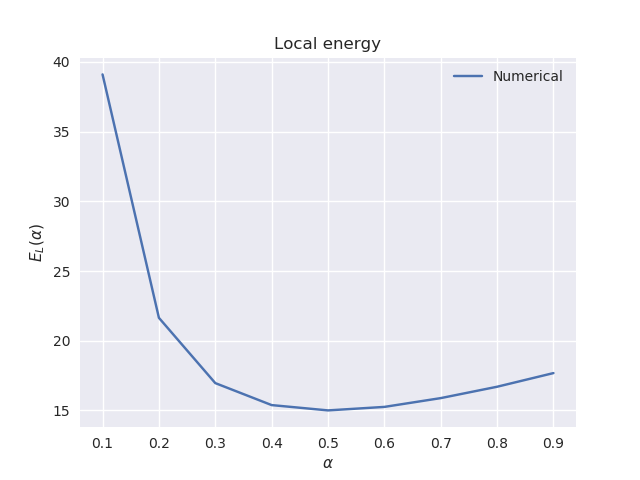
\includegraphics[scale=0.65]{images/energy.png}
    \caption{The local energy for various $\alpha$'s in the interval $\alpha\in[0.1,0.9]$ without interaction. The measure is done with $1e6$ Monte Carlo cycles and the spherical harmonic oscillator trap. }
    \label{fig:energy}
\end{figure} 

\begin{figure} [H]
    \centering
    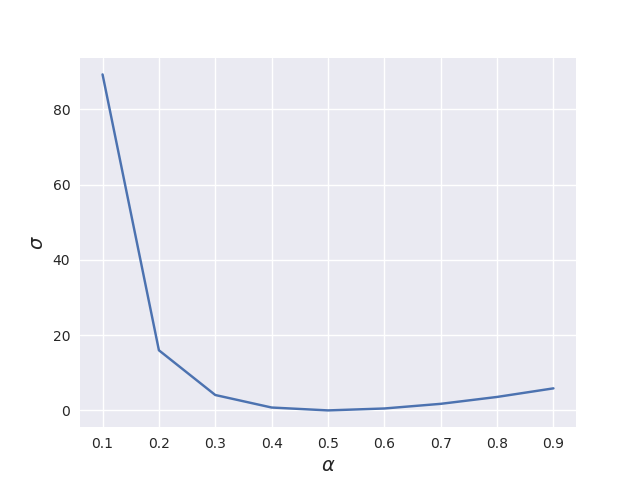
\includegraphics[scale=0.65]{images/variance.png}
    \caption{This variance was found simultaneously with the local energy plotted in figure (\ref{fig:energy}), and was conducted for $\alpha$'s in the interval $\alpha\in[0.1,0.9]$ without interaction. The measure is done with $1e6$ Monte Carlo cycles and the spherical harmonic oscillator trap. }
    \label{fig:variance}
\end{figure} 

\begin{figure}[h] % Do not use only [h] in real documents.
	\begin{minipage}[t]{.45\linewidth}
		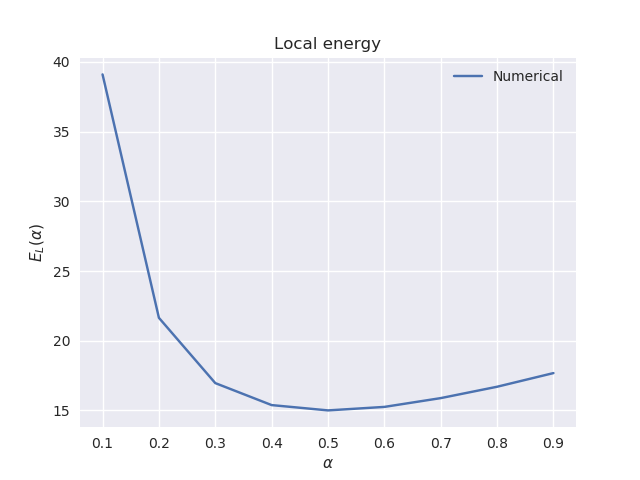
\includegraphics[width=\linewidth]{images/energy.png}
		\caption{Subfigure 1}
	\end{minipage}\hfill
	\begin{minipage}[b]{.45\linewidth}
		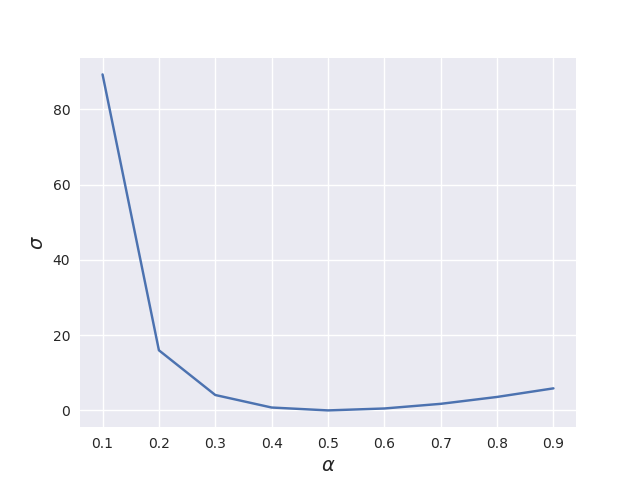
\includegraphics[width=\linewidth]{images/variance.png}
		%\caption{Subfigure 2}
	\end{minipage}
	\caption{Subfigure 3}
\end{figure}

\subsection{Standard Metropolis vs. Importance sampling}
We want to see if the importance sampling really converges faster, and compare the energy with respect to the number of cycles. The interaction is still turned off, and we study 10 particles in 3 dimensions in the minimum point. \\

\begin{figure} [H]
    \centering
    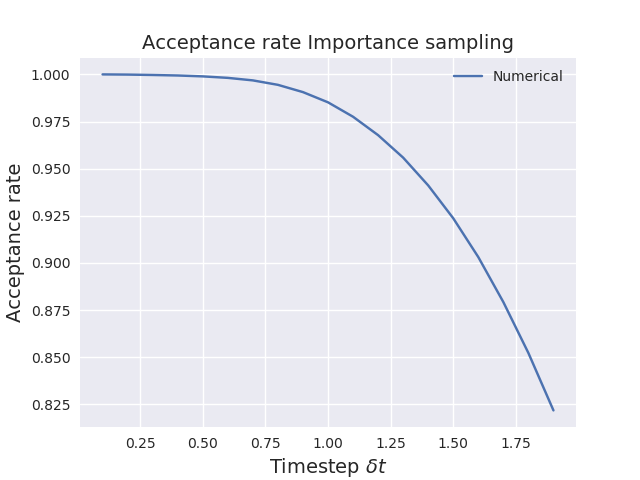
\includegraphics[scale=0.65]{images/acceptance_IS.png}
    \caption{Add caption}
    \label{fig:acceptance_IS}
\end{figure} 

\begin{figure} [H]
    \centering
    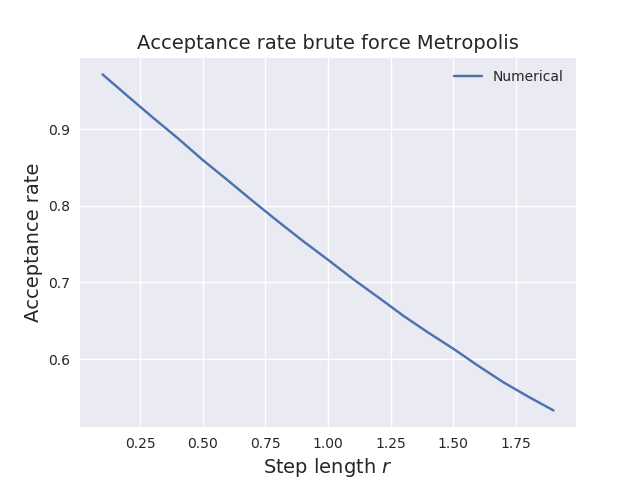
\includegraphics[scale=0.65]{images/acceptance_BF.png}
    \caption{Add caption}
    \label{fig:acceptance_BF}
\end{figure} 

\subsection{VMC with repulsive interaction}
In table \ref{tab:EL_calc_repulsive_pot}, the results from the calculation of the elliptical trap are presented. The variational parameter $\alpha$ was varied manually to find the minimum of the local energy $E_L$.

\begin{table} [H]
	\centering
	\caption{The local energy $E_L$ calculated for different $\alpha$, with $a=0.0043$  with hard-sphere interaction,  elliptical trap and $\beta=2.82843$, with the brute force algorithm with analytical local energy calculation.  The calculations are run in three dimentions with $1e6$ Monte Carlo cycles}
	\begin{tabularx}{\textwidth}{X|XXXXX} \hline
		\label{tab:EL_calc_repulsive_pot}
		$N$ & $\alpha$ = 0.2 & $\alpha$ = 0.3  & $\alpha$ = 0. 35 & $\alpha$ = 0. 4 & $\alpha$ = 0. 5   \\ \hline
		1 & 1.96397 & 1.70441  & 1.68752 & 1.70148 & 1.79225\\
		10 & 19.6679 & 17.1322 & 16.9584 &17.1359 & 18.0973\\
		100 & 255.34 & 253.248 & 262.777 & 275.639 & 307.241\\ \hline
	\end{tabularx}
\end{table}

\subsection{One-body densities}

\begin{figure} [H]
    \centering
    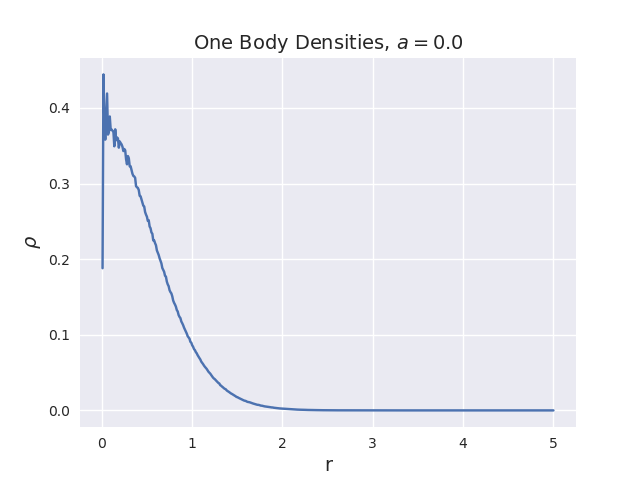
\includegraphics[scale=0.65]{images/ob_a_0.png}
    \caption{Add caption}
    \label{fig:ob0}
\end{figure} 

\begin{figure} [H]
    \centering
    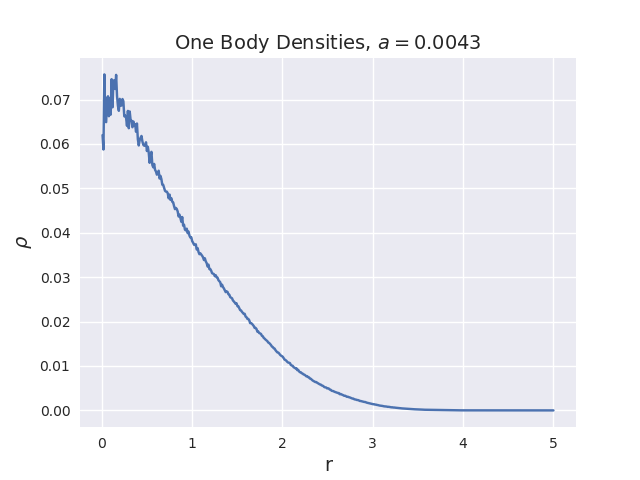
\includegraphics[scale=0.65]{images/ob_a_00043.png}
    \caption{Add caption}
    \label{fig:ob00043}
\end{figure} 

\begin{figure} [H]
    \centering
    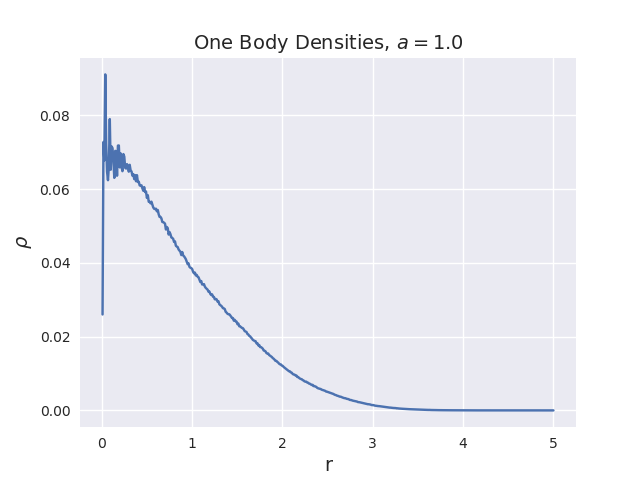
\includegraphics[scale=0.65]{images/ob_a_1.png}
    \caption{Add caption}
    \label{fig:ob1}
\end{figure} 

\section{Discussion}

\section{Conclusion}

\section{Appendix}
\subsection{Appendix A}
\label{appendix_A}

We calculated the analytical expression for the local energy $E_L$, as given by \ref{eq:Local_energy}, for the no-interaction ($a=0$) case for the spherical harmonic oscillator. In this case, the wave trial function for only consists of the one body part, and is thus for $N$ particles given by:

\begin{equation}
	\label{eq:WF_nointeract}
	\Psi_T(\vec{r}) = \prod_i^N e^{-\alpha(x_i^2 + y_i^2 + \beta z_i^2)}
\end{equation}

We now want to calculate the analytical expressions for $E_L$ for one particle and one dimention, and $N$ particles and three dimentions.

\subsubsection{One particle, one dimention}

From \ref{eq:WF_nointeract}, the trial wave function for one particle and one dimention is as follows:

\begin{equation}
	\Psi_T(x) = e^{-\alpha x^2} 
\end{equation}

In the Hamiltonian, the Laplace-operator reduces to the partial derivative in the x-direction, $\frac{\partial^2 }{\partial x^2}$, and $E_L$ is 

\begin{equation}
\begin{aligned}
E_L(x) &=  \frac{1}{\Psi_T(x)}\hat{H}\Psi_T(x) \\ 
			 & =  e^{\alpha x^2} (-\frac{\hbar^2}{2m}\frac{\partial^2 }{\partial x^2} + \frac{1}{2} m \omega_{HO}^2 x^2) e^{-\alpha x^2}  \\
			 & = e^{\alpha x^2} [-\frac{\hbar^2}{2m}\frac{\partial^2 }{\partial x^2} (e^{-\alpha x^2}) + \frac{1}{2} m \omega_{HO}^2 x^2 (^{-\alpha x^2})]
\end{aligned}
\end{equation}

Double differentiation of $ e^{-\alpha x^2}$ yields

\begin{equation}
\frac{\partial^2}{\partial x^2} (e^{-\alpha x^2}) = e^{-\alpha x^2} 2 \alpha (2x^2 -1)
\end{equation}

Inserting this into the expression for $E_L$ gives

\begin{equation}
E_L(\alpha) = -\frac{\hbar^2}{m} \alpha (2x\alpha^2 -1) + \frac{1}{2} m\omega_{HO}^2x^2
\end{equation}

\subsection{$N$ particles, three dimentions}

When extending the non-interaction case to $N$ particles and three dimentions, the trial wave function will take the form listed in \ref{eq:WF_nointeract}, and the Hamiltonian will be as listed in \ref{eq:Hamilton}, with the spherical harmonic oscillator potential $\frac{1}{2}m\omega_{HO}^2r_i^2$, as listed in \ref{eq:V_ext}.

The local energy is then

\begin{equation}
	E_L(\alpha) = \prod_i^N e^{\alpha(x_i^2 + y_i^2 + \beta z_i^2)} \sum_i [ -\frac{\hbar^2}{2m} \nabla_i^2 + \frac{1}{2}m\omega_{HO}^2(x_i^2 + y_i^2 + z_i^2)] \prod_i^N e^{-\alpha(x_i^2 + y_i^2 + \beta z_i^2)}
\end{equation}

Double differentiation of $\Psi_T$ with respect to x gives

\begin{equation}
	\frac{\partial^2}{\partial x^2} (\prod_i e^{-\alpha(x_i^2 + y_i^2 + \beta z_i^2)}) = \prod_i e^{-\alpha(x_i^2 + y_i^2 + \beta z_i^2)} [\sum_{i,j} 4 \alpha^2 x_i x_j -2 \alpha N ]
\end{equation}

Double differentiation with respect to y will give similar answer, while for z there will be a factor $\beta$ difference

\begin{equation}
\frac{\partial^2}{\partial z^2} (\prod_i e^{-\alpha(x_i^2 + y_i^2 + \beta z_i^2)}) = \prod_i e^{-\alpha(x_i^2 + y_i^2 + \beta z_i^2)} [\sum_{i,j} 4 \alpha^2 \beta^2 y_i y_j -2 \alpha \beta N ]
\end{equation}

By including the answers from the differentiations in the x,y and z directions and simplifying the expression results in the following expression for the local energy

\begin{equation}
\begin{aligned}
	E_L(\alpha) & = -\frac{\hbar^2}{2m} N [ \sum_{i,j} 4 \alpha^2 x_i x_j + \sum_{i,j} 4 \alpha^2 y_i y_j + \sum_{i,j} 4 \alpha^2 \beta^2 z_i z_j] +  \\ & \frac{2 \hbar^2}{m}\alpha N^2 + \sum_i \frac{1}{2}m\omega_{HO^2}(x_i^2 + y_i^2 + z_i^2) + \frac{\hbar^2}{m}\beta \alpha N^2
\end{aligned}
\end{equation}


\subsection{Appendix B}
In the theory part we claimed that the Hamiltonian could be written as
\begin{equation}
H=\sum_i\bigg(\frac{1}{2}\Big(-\nabla^2 + x_i^2 + y_i^2 + \gamma^2z_i^2\Big)\bigg)+\sum_{i<j}V_{int}(\vec{r}_i,\vec{r}_j)
\end{equation}
with
\begin{equation*}
\gamma=\frac{\omega_z}{\omega_{HO}}
\end{equation*}
for an elliptical harmonic oscillator potential with repulsive interaction. All the quantities in the expression are scalled, such that it is dimensionless. The energy ($H$) is scalled with respect to $\hbar\omega_{HO}$, while the length is scalled with respect to the characteristic length of the trap, $a_{HO}=(\hbar/m\omega_{HO})^{1/2}$. Let us start from scratch, where the unscalled Hamiltonian for an elliptical harmonic oscillator reads
\begin{equation*}
H=\sum_i\bigg(-\frac{\hbar^2}{2m}\nabla_i^2+\frac{1}{2}m\Big(\omega_{HO}^2(x_i^2+y_i^2)+\omega_z^2z_i^2\Big)\bigg)+\sum_{i<j}V_{int}(\vec{r}_i, \vec{r}_j).
\end{equation*}
We then scale the entire equation with respect to $\hbar\omega_{HO}$
\begin{equation*}
\frac{H}{\hbar\omega_{HO}}=\sum_i\bigg(-\frac{\hbar}{2m\omega_{HO}}\nabla_i^2+\frac{1}{2}\frac{m}{\hbar}\omega_{HO}(x_i^2+y_i^2)+\frac{1}{2}\frac{m}{\hbar}\frac{\omega_z^2}{\omega_{HO}}z_i^2\bigg)+\sum_{i<j}V_{int}(\vec{r}_i, \vec{r}_j)
\end{equation*}
where we can take $H'=H/\hbar\omega_{HO}$ as the dimensionless energy. Further we scale the all the lengths in the same way
\begin{equation*}
x_i^2=(x_i')^2\cdot a_{HO}^2=(x_i')^2\cdot\frac{\hbar}{m\omega_{HO}},
\end{equation*}
and we finally obtain
\begin{equation}
H'=\sum_i\frac{1}{2}\bigg(-\nabla_i^2+(x_i')^2+(y_i')^2+\frac{\omega_z^2}{\omega_{HO}^2}(z_i')^2\bigg)+\sum_{i<j}V_{int}(\vec{r}_i, \vec{r}_j).
\end{equation}
which is the Hamiltonian that we were hunting.
\end{document}
